% Copyright 2019 Clara Eleonore Pavillet

% Author: Clara Eleonore Pavillet
% Description: This is an unofficial Oxford University Beamer Template I made from scratch. Feel free to use it, modify it, share it.
% Version: 1.0

\documentclass{beamer}
% Load Packages
\usepackage[utf8]{inputenc}
\usepackage{xcolor}
\usepackage{tikz}
\usetikzlibrary{positioning,calc}
\usepackage{graphicx}
\usepackage{hyperref}
\usepackage{amsmath}
\usepackage{listings}
\usepackage{fontawesome}
\usepackage{bm}

% Define Commands
\newcommand*{\ClipSep}{0.06cm} %To adjust footer logo
\newcommand{\E}{\mathrm{e}\,} %\def\I{e} % used to defined e for exp(x), see later what it should be
\newcommand{\ud}{\mathrm{d}}
\lstset{numbers=left, numberstyle=\tiny, stepnumber=1,firstnumber=1,breaklines=true,
    numbersep=5pt,language=Python,
    stringstyle=\ttfamily,
    basicstyle=\footnotesize, 
    showstringspaces=false
}

\usetheme{oxonian}

\title{ Bayesian Inference of COVID-19 spreading rates in South Africa - A summary}
\titlegraphic{
\includegraphics[width=2cm]{Theme/Logos/OxfordLogoV1.png}}
\author{Jonas Wildberger}
\institute{University of Oxford}
\date{} %\today
\bibliographystyle{alpha}

\begin{document}

{\setbeamertemplate{footline}{} 
\frame{\titlepage}}

\section*{Outline}\begin{frame}{Outline}\tableofcontents\end{frame}

\section{Problem Description}
    \begin{frame}[plain]
        \vfill
      \centering
      \begin{beamercolorbox}[sep=8pt,center,shadow=true,rounded=true]{title}
        \usebeamerfont{title}\insertsectionhead\par%
        \color{oxfordblue}\noindent\rule{10cm}{1pt} \\
       
      \end{beamercolorbox}
      \vfill
  \end{frame}


\begin{frame}{Problem Description}
\begin{itemize}
	\item<1-> Limited data at the beginning of the pandemic made it difficult to grasp the dynamic of the spread
	\begin{itemize}
		\item<1-> How to account for the high uncertainty in model parameters?
	\end{itemize}
	\item<2-> How to analyse the efficacy of non-pharmaceutical interventions to minimise the spread of COVID-19?	
\end{itemize}
	
	\begin{center}
		\visible<3->{Bayesian inference for the rescue!}
	\end{center}
	 


\end{frame}
\section{Model}
\begin{frame}[plain]
\vfill
\centering
\begin{beamercolorbox}[sep=8pt,center,shadow=true,rounded=true]{title}
	\usebeamerfont{title}\insertsectionhead\par%
	\color{oxfordblue}\noindent\rule{10cm}{1pt} 
	
\end{beamercolorbox}
\vfill
\end{frame}
\begin{frame}{S(E)IR}
	\begin{figure}
	
	\centering
	
\includegraphics[width=0.8\textwidth]{V1}
	\caption{SEIR model \cite{Bayes}}
\end{figure}
\begin{columns}
	\begin{column}{0.5\textwidth}
		\begin{align*}
		\visible<2->{
			\frac{dS}{dt} & = - \frac{\lambda S I }{N} \\
			\frac{dE}{dt} & = \frac{\lambda SI }{N} - \sigma E \\
			\frac{dI}{dt} & = \sigma E - \mu I \\
			\frac{dR}{dt} & = \mu I}
		\end{align*}
	\end{column}
	\begin{column}{0.5\textwidth}
		\begin{itemize}
			\small
			\item<3-> Basic reproductive number $R_0 = \frac{\lambda}{\mu}$  
			\item<3-> Delay $D$ in becoming infected ($I^\text{new}$) and being reported 
			\item<3-> $\lambda$ time-varying with change points corresponding to NIPs 
		\end{itemize}
	\end{column}
\end{columns}

\end{frame}


\begin{frame}{Bayesian model}

\begin{figure}
	\centering
	\visible<1->{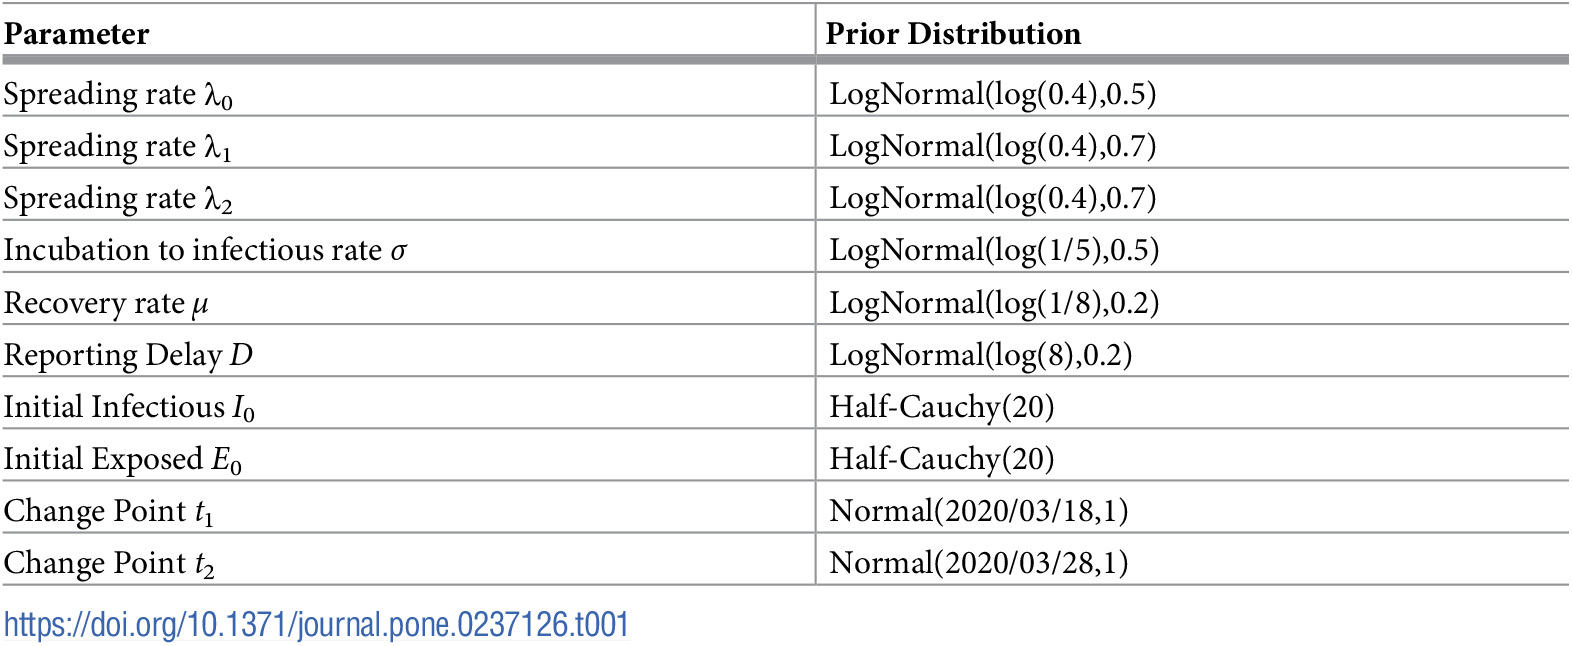
\includegraphics[width=0.8\textwidth]{V2}}
	%\caption{Illustration of Catastrophic Forgetting \cite{zenke2017continual}}
\end{figure}
\begin{itemize}
	\footnotesize
	\item<2-> Likelihood function Student-T distribution
	\item<3-> Initial $R_0 =3.278$ (CI[2.715, 3.73])
	\item<4-> Hamiltonian Monte Carlo (HMC) method to sample from posterior distribution
	
	\begin{itemize} 	
		\item<4 -> No-U-Turn Sampling (NUTS)
		\item<4-> 5000 samples with 1000 burn-in
	\end{itemize}
\end{itemize}
	\note{LogNormal for lambda, sigma s.t. R0 - 3.2 literature value, sigma mean incubation time 5 days, spreading rates increased varaince to keep weaklz informative, weakly infromative half-cauchy distributions for i}

\end{frame}
\section{Results}
\begin{frame}{Results I}
	\begin{figure}
		
		\centering
		\visible<1->{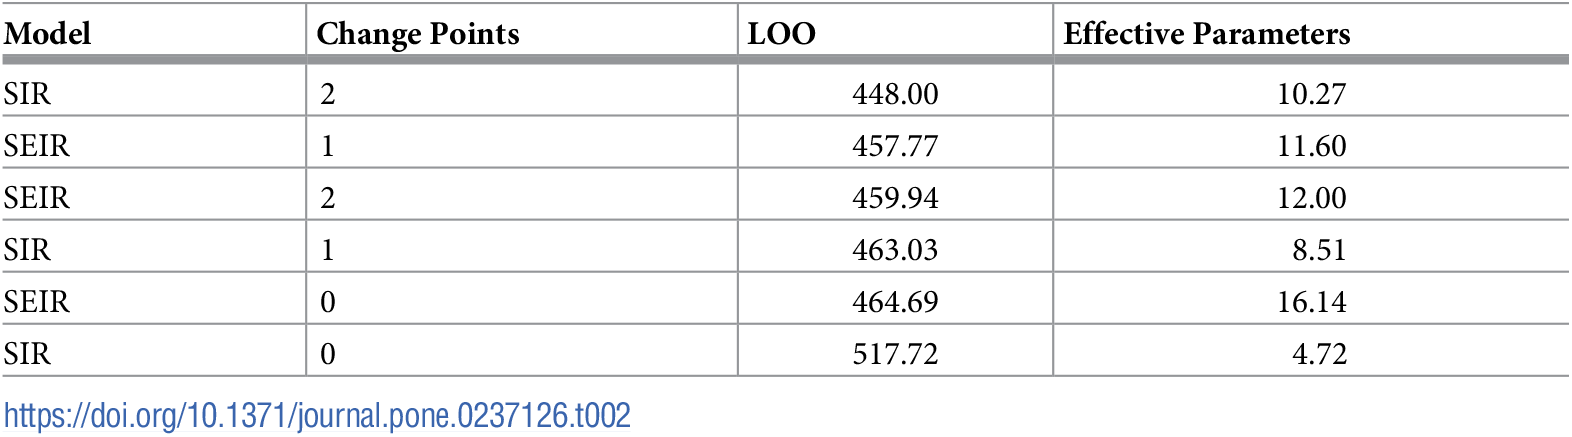
\includegraphics[width=\textwidth]{V3}}
		%\caption{Illustration of Catastrophic Forgetting \cite{zenke2017continual}}
	\end{figure}
	\begin{itemize}
		\item<2-> SIR model with two change points yields lowest LOO cross entropy loss
		
	\end{itemize}
		
\end{frame}
\begin{frame}
	\begin{figure}
		\centering
		\visible<1->{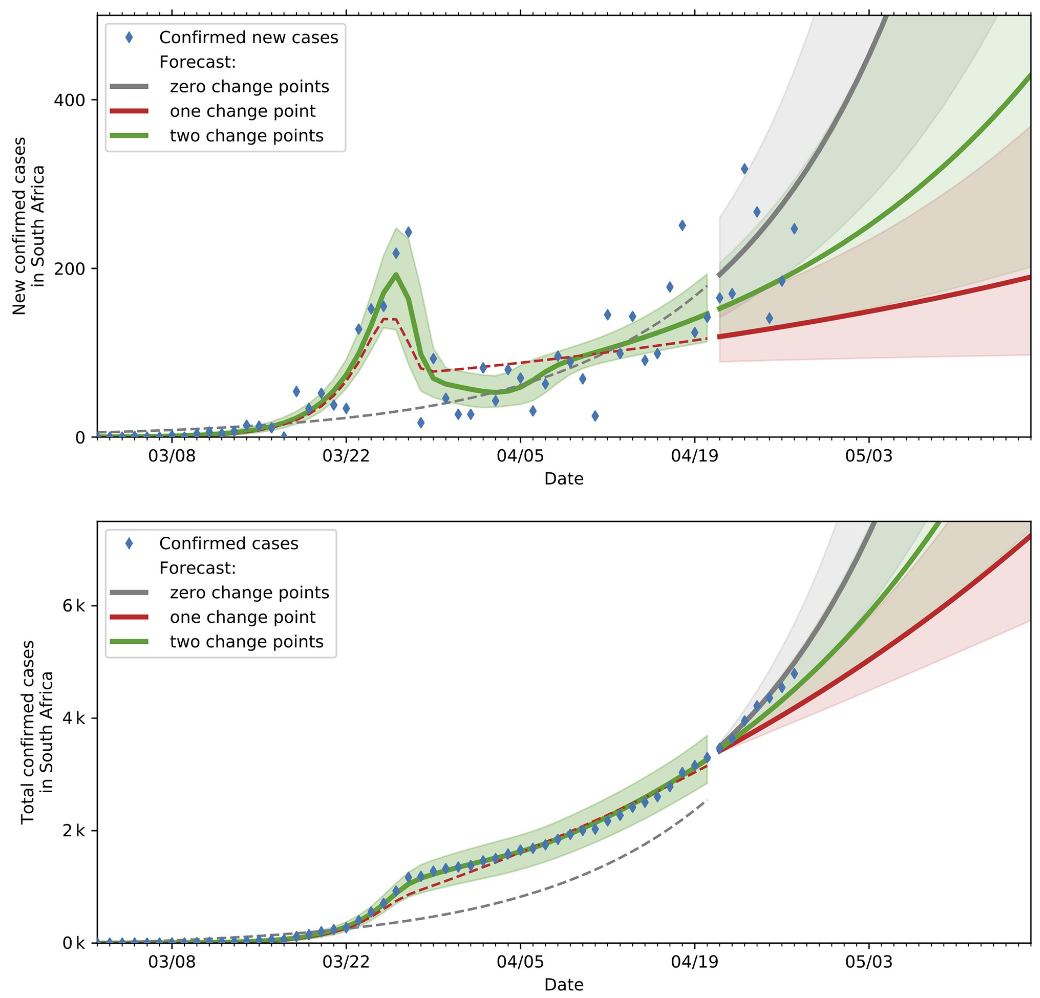
\includegraphics[width=0.8\textwidth]{V4}}
		%\caption{Illustration of Catastrophic Forgetting \cite{zenke2017continual}}
	\end{figure}
\end{frame}

\begin{frame}{Results II}
	
	\begin{columns}
		\begin{column}{0.65\textwidth}
			\begin{figure}
			
			\centering
			\visible<1->{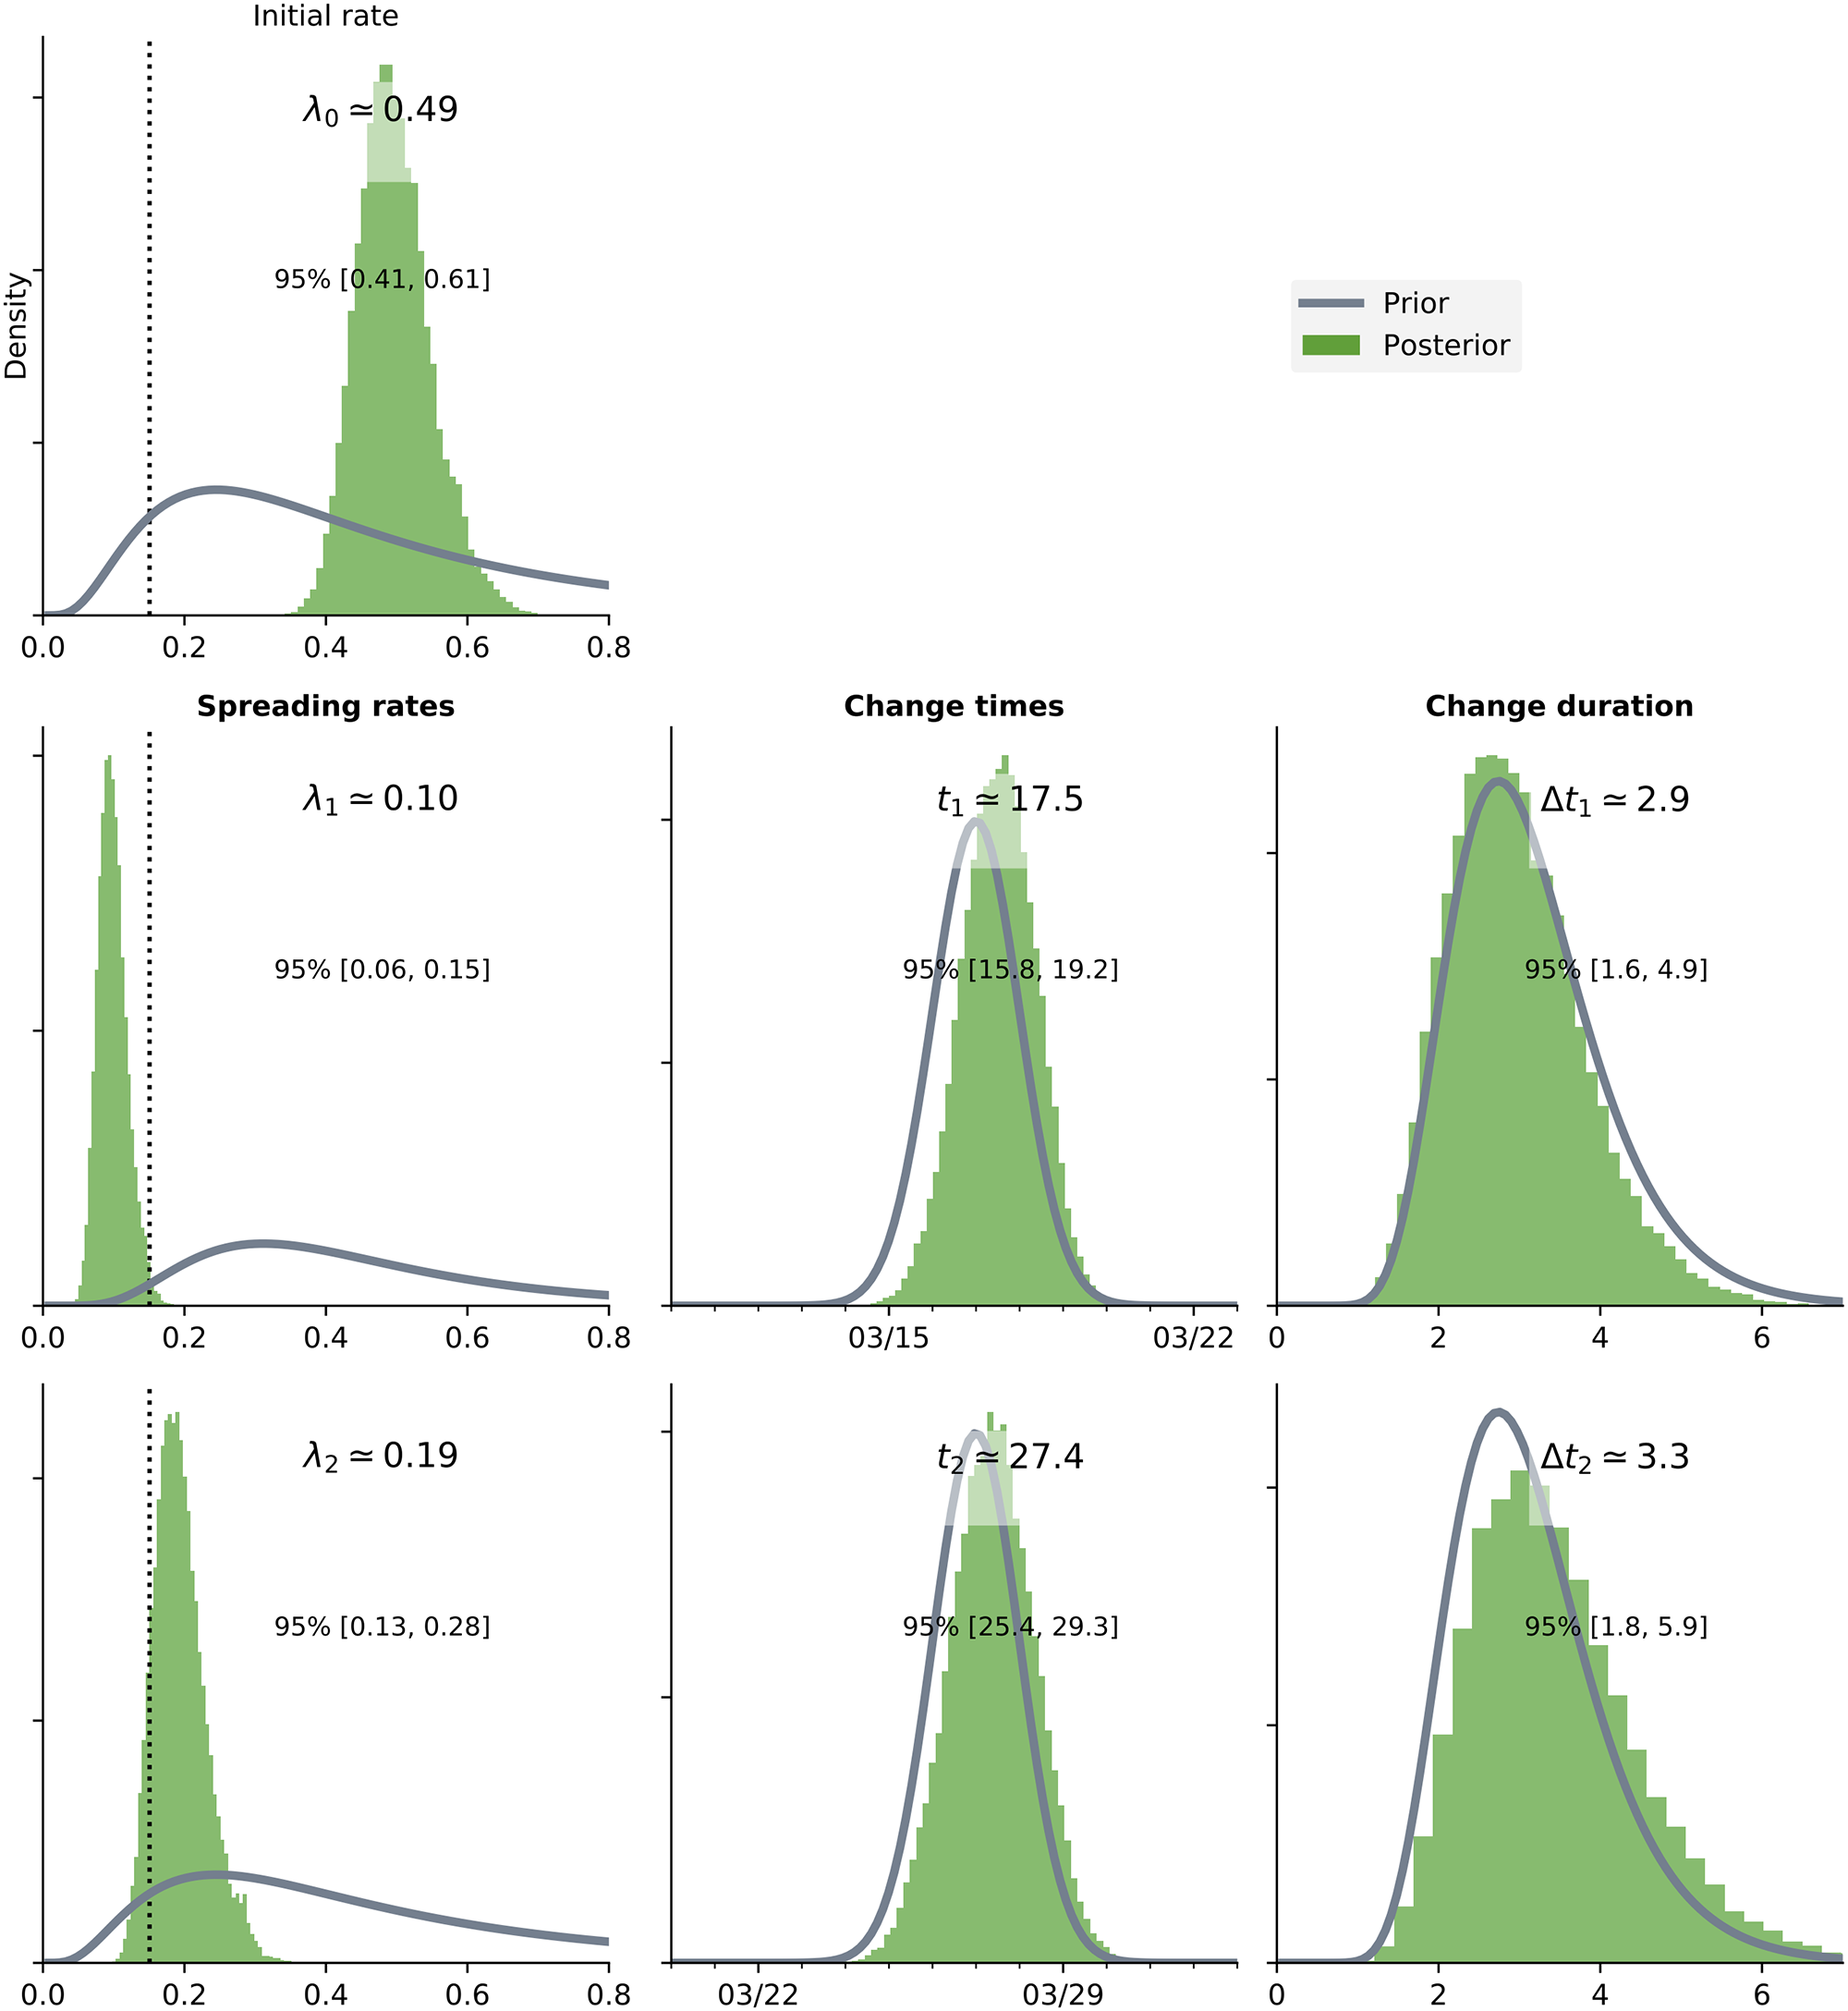
\includegraphics[width=0.8\textwidth]{V5}}
			%\caption{Illustration of Catastrophic Forgetting \cite{zenke2017continual}}
			\end{figure}
		\end{column}
		\begin{column}{0.5\textwidth}
			\begin{itemize}
				\footnotesize
				\item<2-> Change points peak on 18/03 (travel ban, social distancing) and 28/03 (mass testing) 
				\item<3-> Drop of spreading rate by 80\% ($R_0=0.655$ (CI[0.430, 0.960])) and 60\% ($R_0=1.304$ (CI[0.887, 1.7748])) respectively 
				\item<4-> Delay $D\approx 6.848$ including incubation period of 4.537 days, laboratory delay of 2.311 days
				\item<5-> Recovery rate $\mu \approx 0.151$ implies mean infectious period of 6.62 days 
			\end{itemize}
		\end{column}
	\end{columns}
	
\end{frame}




\section{Discussion}
    \begin{frame}[plain]
        \vfill
      \centering
      \begin{beamercolorbox}[sep=8pt,center,shadow=true,rounded=true]{title}
        \usebeamerfont{title}\insertsectionhead\par%
        \color{oxfordblue}\noindent\rule{10cm}{1pt} 
        
      \end{beamercolorbox}
      \vfill
  \end{frame}
\begin{frame}{Discussion}
  \begin{itemize}
  	\item Results confirm the impact of governmental measures to reduce the spread of COVID-19 in South Africa
  	\item<2-> Parameter estimates help quantify the dynamic of the pandemic and account for uncertainty 
  	\item<3-> Assumptions on prior distributions?
  	\item<4-> Take into account local, provincial developments
  \end{itemize}
\end{frame}



\begin{frame}{References}

\bibliography{References}
\end{frame}
\end{document}

